\documentclass[12pt]{article}\usepackage[left=20mm,right=20mm,top=15mm,bottom=20mm]{geometry}

\usepackage[T1]{fontenc}
\usepackage[magyar]{babel}
\usepackage[utf8]{inputenc}
\usepackage[table,xcdraw]{xcolor}

\usepackage{graphicx}
\usepackage{caption}
\usepackage{siunitx}
\usepackage{amsmath}
\usepackage{epstopdf}
\usepackage{multirow}
\usepackage{makeidx}
\usepackage{placeins}
\usepackage{subcaption}
\usepackage{hyperref}

%\DeclareUnicodeCharacter{00A0}{~}

\begin{document}
\begin{titlepage}
\centering
	
\includegraphics[width=0.5\textwidth]{figures/bme_logo_kicsi.eps}\par\vspace{1cm}
	\vspace{1cm}
	\vspace{1.5cm}
	{\huge\bfseries Szoftvertervezés 1. házi feladat \par}
	\vspace{15cm}
	{\huge\itshape Locskai Norbert, Kovács András, Barancsuk Lilla \par}
	\vfill

% Bottom of the page
	{\large \today\par}
\end{titlepage}

\section{Vízió}

\begin{table}[]
\centering
\label{tab:vizio_fejlec}
\begin{tabular}{|l|l|l|l|}
\hline
\rowcolor[HTML]{EFEFEF} 
\multicolumn{1}{|c|}{\cellcolor[HTML]{EFEFEF}\textbf{Verzió}} & \multicolumn{1}{c|}{\cellcolor[HTML]{EFEFEF}\textbf{Dátum}} & \multicolumn{1}{c|}{\cellcolor[HTML]{EFEFEF}\textbf{Leírás}} & \multicolumn{1}{c|}{\cellcolor[HTML]{EFEFEF}\textbf{Készítő}}             \\ \hline
Első verzió                                                   & \today                                                      & Vízió kész                                                   & \begin{tabular}[c]{@{}l@{}}Locskai Norbert\\ Barancsuk Lilla\end{tabular} \\ \hline
                                                              &                                                             &                                                              &                                                                           \\ \hline
\end{tabular}
\end{table}

\subsection{Bevezetés}
A Service4U cég berendezések szervizelésével foglalkozik. Az Device4U nemzetközi cég által
gyártott berendezések szervizelését végzi Magyarországon.
A Service4U vezetői egy olyan számítógépes rendszert szeretnének, mely segítségével képesek
lesznek a raktárban tárolt alkatrész készletet nyomon követni, a rendelés, felhasználás, szállítás, illetve
leltározás folyamatait támogatni.

\subsubsection{Megoldandó probléma}
A programnak nyilván kell tartania a raktárban található összes alkatrészt, illetve azokat az időpontokat, amikor a raktár tartalma változott, a változást, illetve azt, aki a változást bevitte a rendszerbe, valamint segítenie kell a rendelések összeállítását.

Emiatt a rendszernek nyilván kell tartania a cég azon dolgozóit is, akik a programot használják (a vezetőség tagjait, illetve a raktárosokat, akik a rendeléseket átveszik, és az eszközöket kiadják).

Nyilván kell tartania még a szervizelt berendezések típusait, és azok alkatrészeit, valamint képesnek kell lennie frissíteni a berendezések listáját.

A program segítségével a cég vezetőinek legyen lehetősége rendelések összeállítására, illetve azok exportálására többféle formátumban (pdf, xls, txt).
 
Mivel a Service4U minden alkatrészből legalább két darabot kíván raktáron tartani, a programnak értesítenie kell a cég vezetőségét, amennyiben bármely alkatrész száma kettő alá csökken.

Az alkatrészeket a Service4U cég szerelői vételezik ki a raktárból egy-egy berendezés javítása
során. 
A szerelők a kivenni kívánt alkatrészeket munkalapon rögzítik, majd azt átadják a raktárosnak. 
A raktárosnak a rendszer segítségével képesnek kell lennie a kivétel nyilvántartására: az időpont, a szerelő, a raktáros azonosítójának, illetve a kivett alkatrészek rögzítésére.

A szállítást mindig azonos szállító cég végzi, akik adott rendelést mindig egy szállítási egységként szállítják.
A program segítségével a raktárosnak rögzítenie kell tudnia a szállítmány tartalmát és bevételezésének időpontját.

Service4U cég vezető félévente leltározást végeznek a raktárban, amikor elkészítik azt a listát, ami a
raktárban levő alkatrészeket tartalmazza.
A rendszernek alkalmasnak kell lennie arra, hogy az adatbázisban lévő alkatrészeket automatikusan összeszámlálja, valamint a kézi leltárral összevethető formában megjelenítse a számlálás eredményét.


\subsection{Érdekeltek köre - stakeholderek}
\begin{itemize}
\item[] \textbf{vezető: } A vezető végzi az alkatrészek megrendelését, kezdeményezi a leltározást, továbbá bevihet új berendezéseket az adatbázisba. Célja a raktár kiürülésének megakadályozása, valamint a fent említett munkafolyamatok gyorsítása, automatizálása.

\item[] \textbf{szerelő: } A szerelő végzi a gépek javítását, e célból alkatrészeket kér ki a raktárból.  Célja, hogy a szükséges alkatrészek rendelkezésre álljanak, valamint hogy a kivétel gyors legyen.

\item[] \textbf{raktáros: } A raktáros az a személy, aki a szerelőknek kiadja az alkatrészeket, valamint a beszállítóktól átveszi azokat. Emellett a kézi leltározást végzi. Célja, hogy egyszerűen adminisztrálja a raktár tranzakcióit, valamint értesítést kapjon a leltárazás elkezdéséről.

\item[] \textbf{rendszergazda: } A rendszergazda a rendszer karbantartását végzi, valamint ő felelős új munkatársak nyilvántartásának naprakészen tartásáért. Célja, hogy a rendszer egyszerűen karbantartható, visszaállítható és bővíthető legyen.
\end{itemize}

\subsection{Rendszer részei}
\begin{itemize}
\item[] \textbf{adatbázis: } Nyilvántartás, ami tartalmazza a kollégákat, a gépeket, azok alkatrészeit, valamint a gépekben található alkatrészeket, valamint a raktári tranzakciókat, ezen kívül az éves leltár eredményét. A rendszeres biztonsági mentések segítségével az adatbázis állapota bármikor visszaállítható. Megkönnyíti és gyorsítja a cégen belüli adminisztrációt, valamint segíti hiba esetén a rendszer visszaállítását.

\item[] \textbf{grafikus felület (GUI): } A grafikus felhasználói felület megjeleníti a szükséges adatokat, valamint lehetővé teszi új adatok bevitelét a rendszerbe. 
A GUI átlagfelhasználó számára is lehetővé teszi a rendszer használatát, az adatbázisba való adminisztrációt. 

\item[] \textbf{adatbázis--GUI interfész: } Az adatbázist és grafikus felületet összekötő interfész, ami lekérdezéseket hajt végre az adatbázisban, valamint a lekérdezések eredményét és az ezekből származtatott adatokat továbbítja a grafikus felületnek.
Ez az interfész megkönnyíti az adatbázis kezelését.

\item[] \textbf{azonosítófelület: } Az azonosítófelület megakadályozza az illetéktelen hozzáférést. Ennek segítségével beállíthatók a jogosultságok, valamint ellenőrizhető, hogy egyes műveleteket ki és mikor végzett.

\item[] \textbf{lehetőség távoli hozzáférésre: } Távoli elérés lehetőségét biztosító rendszerrész, aminek segítségével a kollégák hálózaton keresztül is kezdeményezhetnek bizonyos műveleteket.

\item[] \textbf{vonalkódleolvasó--vonalkódfeldolgozó: } Beolvassa és értelmezi az alkatrészek vonalkódjait, ezzek egyszerűbbé téve az adminisztrációt.
\end{itemize}

\subsection{Rendszer korlátai, határai}
\subsubsection{A rendszer feladatainak határai}
A rendszer nem felelős a raktár fizikai feltöltéséért--ürítéséért, leltározásáért. Azt a feladatot a raktáros látja el.
Emellett a program nem képes a kollégák adatainak automatikus importálására a céges nyilvántartásból. 
Ezeket az adatokat a rendszergazda kézzel viszi be, és rendel a személyekhez jogosultságokat.
Ezen kívül nem a rendszer feladata a rendelések elküldése, ezeket csak összeállítja, valamint olvasható formában megjeleníti és exportálja.

\subsubsection{Technológiai korlátok}
A cég számítógépparkja technológiai korlátokat állít a rendszer elé.
Szerverként egyetlen gép áll rendelkezésre, amely csak korlátozott számú kérést tud egyszerre kiszolgálni. 
A kollégák által használt számítógépek elavult, asztali gépek korlátos erőforrásokkal, továbbá programok telepítésére és törlésére csak a rendszergazdának van jogosultsága.

\section{Fogalomszótár}
\begin{itemize}
\item[]\textbf{berendezés: } A cég által szervizelt gép.

\item[]\textbf{alkatrész: } A gépek építőelemei, amiket raktárban tárol a cég. 

\item[]\textbf{szerelő: } A gépek szervizelését végzi. Alkatrészeket vesz ki a raktárból.

\item[]\textbf{vezető: } Az az ember, aki felelős az alkatrészek rendeléséért, illetve a leltározás elrendeléséért.

\item[]\textbf{raktáros: } Kezeli a raktárat: kiadja a szerelőnek a neki szükséges alkatrészeket, átveszi a szállító által szállított alkatrészeket, valamint elvégzi a manuális leltárazást.

\item[]\textbf{szállítólevél: } Az a dokumentum, ami tartalmazza az adott szállítmányban található alkatrészek típusait és darabszámát.

\item[]\textbf{munkalap: } Az a dokumentum, ami tartalmazza a javítandó berendezéshez szükséges alkatrészeket. 

\item[]\textbf{rendszergazda: } A cég azon alkalmazottja, aki a kezeli a munkatársak jogosultságait, valamint a rendszer karbantartását végzi.

\item[]\textbf{rendelés: } Az a dokumentum, ami tartalmazza a megrendelni kívánt alkatrészek darabszámát és típusát.

\item[]\textbf{leltározás: } Az a folyamat, amelynek során a tényleges raktárkészletet összehasonlítják a nyilvántartással.

\item[]\textbf{jelentés: } A leltározás során készült dokumentum, ami összehasonlítható formában tartalmazza a fizikai számlálás és az elektronikus nyilvántartás eredményeit.
\end{itemize}

\section{Kiegészítő követelmények leírása}

\begin{table}[]
\centering
\label{tab:srs_fejlec}
\begin{tabular}{|l|l|l|l|}
\hline
\rowcolor[HTML]{EFEFEF} 
\multicolumn{1}{|c|}{\cellcolor[HTML]{EFEFEF}\textbf{Verzió}} & \multicolumn{1}{c|}{\cellcolor[HTML]{EFEFEF}\textbf{Dátum}} & \multicolumn{1}{c|}{\cellcolor[HTML]{EFEFEF}\textbf{Leírás}} & \multicolumn{1}{c|}{\cellcolor[HTML]{EFEFEF}\textbf{Készítő}}             \\ \hline
Első verzió                                                   & \today                                                      & Vízió kész                                                   & \begin{tabular}[c]{@{}l@{}}Locskai Norbert\\ Barancsuk Lilla\end{tabular} \\ \hline
                                                              &                                                             &                                                              &                                                                           \\ \hline
\end{tabular}
\end{table}

\subsection{Funkcionális követelmények}
Mivel a rendszer egy raktár nyilvántartását végzi, ezért szükséges, hogy adatbázis mindig tükrözze a tényleges raktárkészletet, megkönnyítse az adminisztrációt és a leltározást.

\subsection{Használhatóság}
Mivel az egyszerű felhasználók nem jártasak az adatbázis-kezelésben, a grafikus felület ergonomikus és intuitív lehetőséget biztosít ennek kezelésére.

\subsection{Megbízhatóság}
A adatbázisban állapotainak visszaállíthatónak kell lenniük, hiba után is. 
Ezért az adatbázisról rendszeresen (minden munkanapon éjfélkor) mentés készül.
Valamint naplózás segítségével a változások nyomon követhetők.

\subsection{Teljesítmény}
Az adatbázisnak képesnek kell lennie nagyszámú adat tárolására. 
Számszerűen:
\begin{itemize}
\item[•] maximum 10.000 féle alkatrész
\item[•] maximum 10.000 darab alkatrész fajtánként
\item[•] maximum 1000 féle gép
\item[•] egy géphez maximum 1000 alkatrész rendelhető
\end{itemize}

A rendszernek kezelnie kell maximum 10 darab egyidejű hozzáférést. 

\subsection{Támogatottság}
Fontos, hogy az adatbázis bővíthető legyen új kollégákkal, valamint új berendezésekkel.
A cég vállalja a szoftver rendszeres karbantartást, ami félévente esedékes ellenőrzést, hibajavítást jelent.
Valamint lehetőség van telefonos ügyfélszolgálat igénybevételére, illetve hibabejelentésre.

\subsection{Technológiai megkötések}
A GUI-nak a következő böngészőkön a megadott verziószámok fölött kell tudni futnia:
\begin{itemize}
\item[•] Chrome 48.0
\item[•] Mozzilla Firefox 44
\item[•] Internet Explorer 9.0
\item[•] Safari 9.0
\end{itemize}

A cég kis teljesítményű, elavult gépei a szoftvernek korlátos erőforrású környezetben is megfelelően kell működnie. 
A jogosultságok korlátozása miatt a grafikus felületnek böngészőben megjeleníthetőnek kell lennie.
Mivel egyetlen szerver áll rendelkezésre, az adatbázisba befutó kéréseket ennek kell elvárható időn belül (1 s) kiszolgálnia.

\subsection{Interfészek}
A szoftvernek nem szükséges külső rendszerekkel együttműködni.

\section{Use Case modell}
\subsection{Aktorok}
\subsubsection{Elsődleges aktorok}
\begin{itemize}
\item[•] \textbf{vezetők: }  A célja az alkatrészek megrendelése, leltározás kezdeményezése, továbbá új berendezések bevitele az adatbázisba, a raktár kiürülésének mgakadályozása. Elvárása a rendszerrel kapcsolatban, hogy a fent említett folyamatokat automatizáltan, gyorsan végrehajtsa.
 
\item[•] \textbf{szerelő: } A szerelő célja, hogy a szükséges alkatrészekhez a lehető leggyorsabban hozzáférjen, illetve ezek mindig rendelkezésre álljanak.

\item[•] \textbf{raktáros: } A raktáros célja a raktár adminisztációjának gyors, megbízható elvégzése. 
Szeretne időben értesítést kapni a leltár elkezdéséről.

\item[•] \textbf{rendszergazda: } Célja, hogy a rendszer egyszerűen karbantartható, visszaállítható és bővíthető legyen.
\end{itemize}

\subsubsection{Támogató aktorok}
\begin{itemize}
\item[•] \textbf{raktáros: } Célja, hogy a szerelőktől vagy a vezetőségtől érkező kéréseket gyorsan kiszolgálja, valamint egyszerűen intézze az alkatrészek átvételét.
Szeretné, hogy fenti munkafolyamatok jól dokumentáltak legyenek.

\item[•] \textbf{adatbázis: } Adatokat tárol és szolgáltat. Kiszolgálja a beérkező kéréseket.
\end{itemize}

\section{Legfontosabb use case-ek}
\subsection{Rendelés}
\begin{itemize}
\item[] \textbf{azonosító: } UC1

\item[] \textbf{aktorok: } Elsődleges: vezető, támogató: adatbázis.  

\item[] \textbf{érdekeltek: } Vezető: Szeretné a rendszer keretein belül gyorsan összeállítani a szükséges alkatrészek rendelési listáját.

\item[] \textbf{előfeltételek: } Egy adott típusú alkatrész készleteinek növelésére igény merül fel.

\item[] \textbf{hatása: } Rendelési fájl generálódik, ami tarmazza a rendelt alkatrészek listáját.

\item[] \textbf{alap forgatókönyv: }
\begin{enumerate}
\item Valamelyik típusú alkatrész száma kettő alá csökken.
\item A vezető bejelentkezik.
\item A vezető megnyitja a rendelésösszeállító ablakot.
\item A vezető alkatrészt ad hozzá a rendeléshez, beállítja a rendelni kívánt alktrész darabszámát. \\
\textit{A vezető az előző lépést a rendelés teljes összeállításáig ismétli.}
\item A vezető exportálja az elkészült listát valamilyen formátumban (pdf, szöveg, táblázat).
\item A vezető kilép a rendszerből.
\end{enumerate}

\item[] \textbf{alternatív forgatókönyv: }
\begin{enumerate}
\item Igény merül fel valamilyen típusú alkatrészre.
\item A vezető bejelentkezik.
\item A vezető megnyitja a rendelés-összeállító ablakot.
\item A vezető alkatrészt ad hozzá a rendeléshez, beállítja a rendelni kívánt alkatrész darabszámát.
\textit{A vezető az előző lépést a rendelés teljes összeállításáig ismétli.}
\item A vezető exportálja az elkészült listát valamilyen formátumban (pdf, szöveg, táblázat).
\item A vezető kilép a rendszerből.
\end{enumerate}

\item[] \textbf{különleges követelmények: } A rendelést csak vezetői jogosultsággal rendelkező személy végezheti.

\item[] \textbf{technológiai variánsok: } \\Az elkészült rendelés exportálható többféle fájlformátumban:
\vspace*{-3mm}
\begin{itemize}
\item[•] xls
\item[•] pdf
\item[•] txt
\end{itemize}
\end{itemize} 

\begin{figure}[!h]
    \centering
        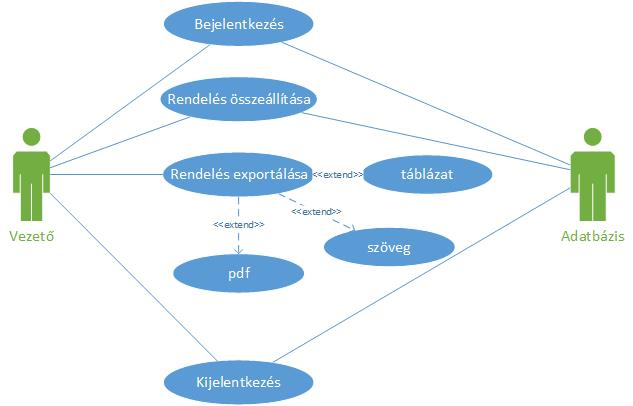
\includegraphics[width=0.7\textwidth]{figures/rendeles_UC.jpg}
        \caption{A rendelés use case diagramja.}
\end{figure}

\begin{figure}[!h]
    \centering
        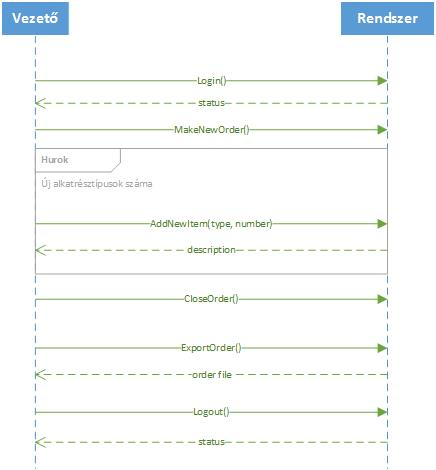
\includegraphics[width=0.7\textwidth]{figures/rendeles_SD.jpg}
        \caption{A rendelés szekvenciadiagramja.}
\end{figure}

\subsection{Leltárazás}
\begin{itemize}
\item[] \textbf{azonosító: } UC2
\item[] \textbf{aktorok: } Kezdeményező: vezető, támogató: adatbázis, raktáros.

\item[] \textbf{érdekeltek: }
\vspace*{-3mm}
\begin{itemize}
\item[•] vezető: Célja a leltár automatizált végrehajtása, illetve a fizikai leltározás kezdeményezése. Fontos neki, hogy a folyamat végén egyetlen, áttekinthető dokumentumban láthassa az eredményt.

\item[•] raktáros: Célja, hogy időben értesüljön arról, hogy el kell kezdenie a fizikai leltározást. 

\item[•] adatbázis
\end{itemize}

\item[] \textbf{előfeltételek: } A folyamat előfeltétele, hogy az utolsó leltár óta félév eltelt, illetve vezetői jogosultsággal rendelkező felhasználó kezdeményezze.

\item[] \textbf{hatása: }
A folyamat végén dokumentum készül, ami tartalmazza a fizikai leltár eredményét, illetve az elektronikus adatbázis összesítését.

\item[] \textbf{alap forgatókönyv: }
\begin{enumerate}
\item A vezető bejelentkezik a rendszerbe.
\item A vezető kezdeményezi a leltár elkezdését.
\item A raktárkészletet a rendszer befagyasztja.
\item A rendszer automatikusan összegzi az adatbázisban található alkatrészeket.
\item A rendszer értesítést küld a raktárosnak a leltár elkezdéséről.
\item A raktáros elvégzi a fizika leltározást.
\item A raktáros beviszi a rendszerbe a számlálás eredményét.
\item A rendszer jelentést készít a két eredményből.
\item A vezető kilép a rendszerből.
\end{enumerate}
\end{itemize} 

\begin{figure}[!h]
    \centering
        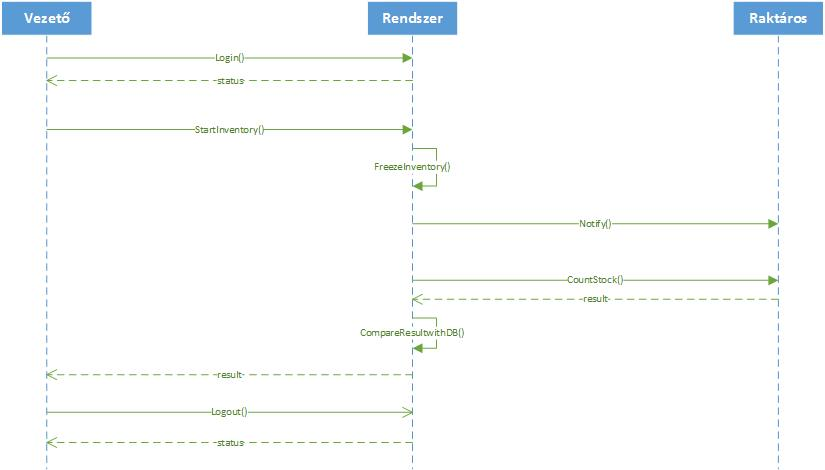
\includegraphics[width=0.9\textwidth]{figures/leltarazas_SD.jpg}
        \caption{A leltározás szekvenciadiagramja.}
\end{figure}

\begin{figure}[!h]
    \centering
        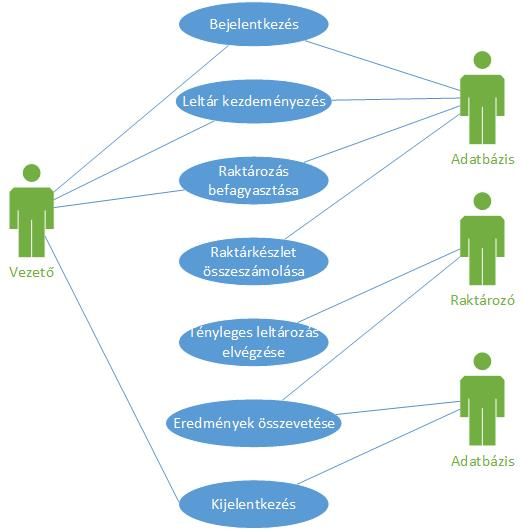
\includegraphics[width=0.7\textwidth]{figures/leltarazas_UC.jpg}
        \caption{A leltározás use case diagramja.}
\end{figure}

\FloatBarrier
\subsection{Alkatrész kiadása}
\begin{itemize}
\item[] \textbf{azonosító: } UC3
\item[] \textbf{aktorok: } Elsődleges: szerelő, támogató: adatbázis, raktáros, háttér: vezető.

\item[] \textbf{érdekeltek: }
\vspace*{-3mm}
\begin{itemize}
\item[•] szerelő: A szerelő célja, hogy a lehető leggyorsabban kézhez kapja a szükséges alkatrészeket.
\item[•] raktáros: Célja, hogy a lehető legkevesebb adminisztrációval ki tudja szolgálni a szerelőt.
\item[•] vezető: Érdekelt abban, hogy a szükségesnél több alkatrész ne kerüljön felhasználásra.
\end{itemize}

\item[] \textbf{előfeltételek: } Szerelő kézhez kapja a munkalapot.

\item[] \textbf{hatása: } Szerelő megkapja a szükséges alkatrészeket, a kiadás rögzítésre kerül az adatbázisban.

\item[] \textbf{alap forgatókönyv: }
\begin{enumerate}
\item Szerelő átadja a munkalapot a raktárosnak.
\item A raktáros beviszi a munkalapon lévő adatokat a rendszerbe.
\item A rendszer megjeleníti a szükséges alkatrészeket.
\item A raktáros összegyűjti és vonalkód-leolvasóval beolvassa a megjelenített alkatrészeket.
\item A rendszer frissíti az adatbázist.
\item A raktáros kiadja az alkatrészeket. \\
\textit{A folyamat a szerelőnél lévő összes munkalapra ismétlődik.}
\end{enumerate}

\item[] \textbf{alternatív forgatókönyv:} \\
Ha adott alkatrészből nem áll rendelkezésre megfelelő mennyiség, akkor a folyamat a következőképpen módosul a 3. ponttól kezdve:
\begin{enumerate}
\item A rendszer kiírja, hogy adott alkatrész hiányzik.
\item A raktáros törli az adott munkalapot.
\item A raktáros visszaadja a munkalapot a szerelőnek.
\item A rendszer értesítést küld a vezetőnek az alkatrésztípus hiányáról.
\end{enumerate}

\item[] \textbf{különleges követelmények: } Vonalkódleolvasó eszköz.
\end{itemize} 

\begin{figure}[!h]
    \centering
        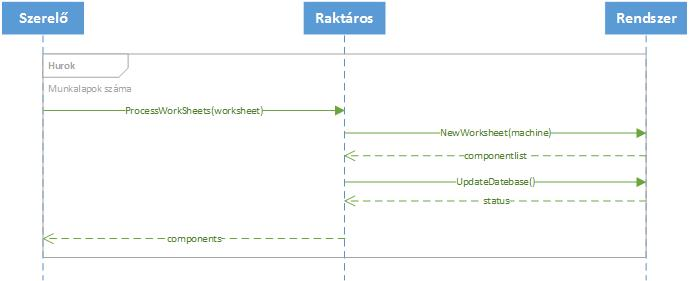
\includegraphics[width=0.9\textwidth]{figures/alkatresz_kiadas_SD.jpg}
        \caption{Az alkatrész kiadás szekvenciadiagramja.}
\end{figure}

\begin{figure}[!h]
    \centering
        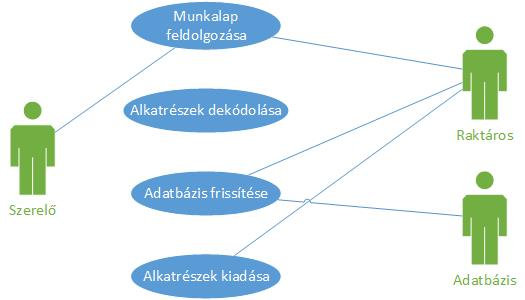
\includegraphics[width=0.9\textwidth]{figures/alkatresz_kiadas_UC.jpg}
        \caption{Az alkatrész kiadás use case diagramja.}
\end{figure}


\FloatBarrier
\subsection{User nyilvántartás}
\textbf{azonosító: } UC4 \\
A rendszergazda a rendszerbe belépve beviszi a számára kialakított beviteli felületen az új munkatársak adatait, jogosultságokat rendel hozzájuk, módosításokat végez, vagy törli őket. 
A folyamat eredményeképpen a kollégák adatainak változásai megjelennek az adatbázisban.

\subsection{Bejelentkezés}
\textbf{azonosító: } UC5 \\
A rendszerbe bejelentkezhet raktáros, rendszergazda és vezető is.
Bejelentkezéskor meg kell adni az egyedi azonosítót valamint a jelszót.
A bejelentkezés eredményeképpen a felhasználó a jogosultsági szintjének megfelelő műveletek végrehajtására lesz képes.

\subsection{Automatikus értesítés}
\textbf{azonosító: } UC6 \\
Az automatikus értesítést a rendszer küldi a vezetőknek, ha egy adott típusú alkatrész darabszáma a raktárban kettő alá csökken.
A rendszer minden adatbázis-módosításkor ellenőrzi a darabszámokat, és hiány esetén értesítést küld a vezetőknek, akik ezt a rendszerbe belépve megkapják.

\subsection{Új berendezés bevitele}
\textbf{azonosító: } UC7 \\
Ha módosul a szervizelt berendezések listája, a vezetőség az adatbázist belépés után kiegészítheti az új berendezéssel, valamint a hozzá szükséges alkatrészek listájával.

\subsection{Backlog lekérdezése}
\textbf{azonosító: } UC8 \\
A vezetőség ellenőrzés céljából lekérheti bizonyos tranzakciók naplóját. 
A folyamat eredményeképpen a rendszer áttekinthető formában megjeleníti a kívánt időpontban naplózott bejegyzéseket.

\subsection{Megrendelés átvétele}
\textbf{azonosító: } UC9 \\
A raktáros átveszi az érkezett csomagot a szállítólevéllel együtt, beviszi a rendszerbe az új szállítmányt, majd egyenként leolvassa a szállítmányba tartozó alkatrészek vonalkódját.
Ezután elhelyezi őket a raktárban.
A folyamat végén megnő a raktárban és a nyilvántartásban jelen lévő alkatrészek száma.

\subsection{Biztonsági mentés készítése}
\textbf{azonosító: } UC10 \\
Minden munkanapon éjfélkor a rendszer automatikusan biztonsági mentést készít az adatbázis aktuális állapotáról.
Az ennek eredményeképpen létrejövő fájl segítségével a rendszergazda hiba esetén vissza tudja állítani a rendszer korábbi állapotát.

\subsection{Rendszer visszaállítása}
\textbf{azonosító: } UC11 \\
Hiba fellépése esetén a rendszergazda egy biztonsági mentés segítségével a rendszert vissza tudja vinni korábbi állapotába.

\end{document}